%%Berichtvorlage für EDBV WS 2014/2015

\documentclass[paper=A4, deutsch]{scrartcl}
\usepackage[ngerman]{babel}
\usepackage[utf8]{inputenc}
\usepackage{algorithmic}
\usepackage{algorithm}
\usepackage{graphicx}
\usepackage{amsmath,amssymb}
\usepackage{subcaption}
\captionsetup{compatibility=false}
\usepackage{multirow}
\usepackage{color}
\usepackage[]{geometry}
\usepackage{textcomp}
\usepackage{soul}

\newcommand\tab[1][1cm]{\hspace*{#1}}

\begin{document}


%%------------------------------------------------------
%% Ab hier tragt ihr eure Daten und Ergebnisse ein:
%%------------------------------------------------------

\title{Lib-Indexer} %%Projekttitel hier eintragen

\subtitle{EDBV WS 2019/2020: AG\_C\_3} %%statt XX Arbeitsgruppenbezeichnung hier eintragen (zB.: A1)


%%Namen und Matrikelnummern der Gruppenmitglieder hier eintragen
\author{Anand Eichner (11808244)\\
Laurenz Edmund Fiala (11807869)\\
Anna Nieto-Berezhinskaya (01223066)\\
Aleksandar Vucenovic (01635282)}



%%------------------------------------------------------

\maketitle


%%------------------------------------------------------
\section{Gewählte Problemstellung}
(1-1,5 Seiten)\\
entspricht dem (aktualisierten) Konzept
\subsection{Ziel}
Das Projekt soll Bücher in einem Bücherregal erkennen, in Bücher-Koordinaten umwandeln und nach ihrem Label abspeichern.

\subsection{Eingabe}
JPG-Bild eines Bücherregals mit Büchern, auf denen eindeutige TU-Bibliotheks-Labels (schwarz-auf-weiß) kleben.

\subsection{Ausgabe}
visuell:\\
\\
\begin{figure}[H]
 \centering
 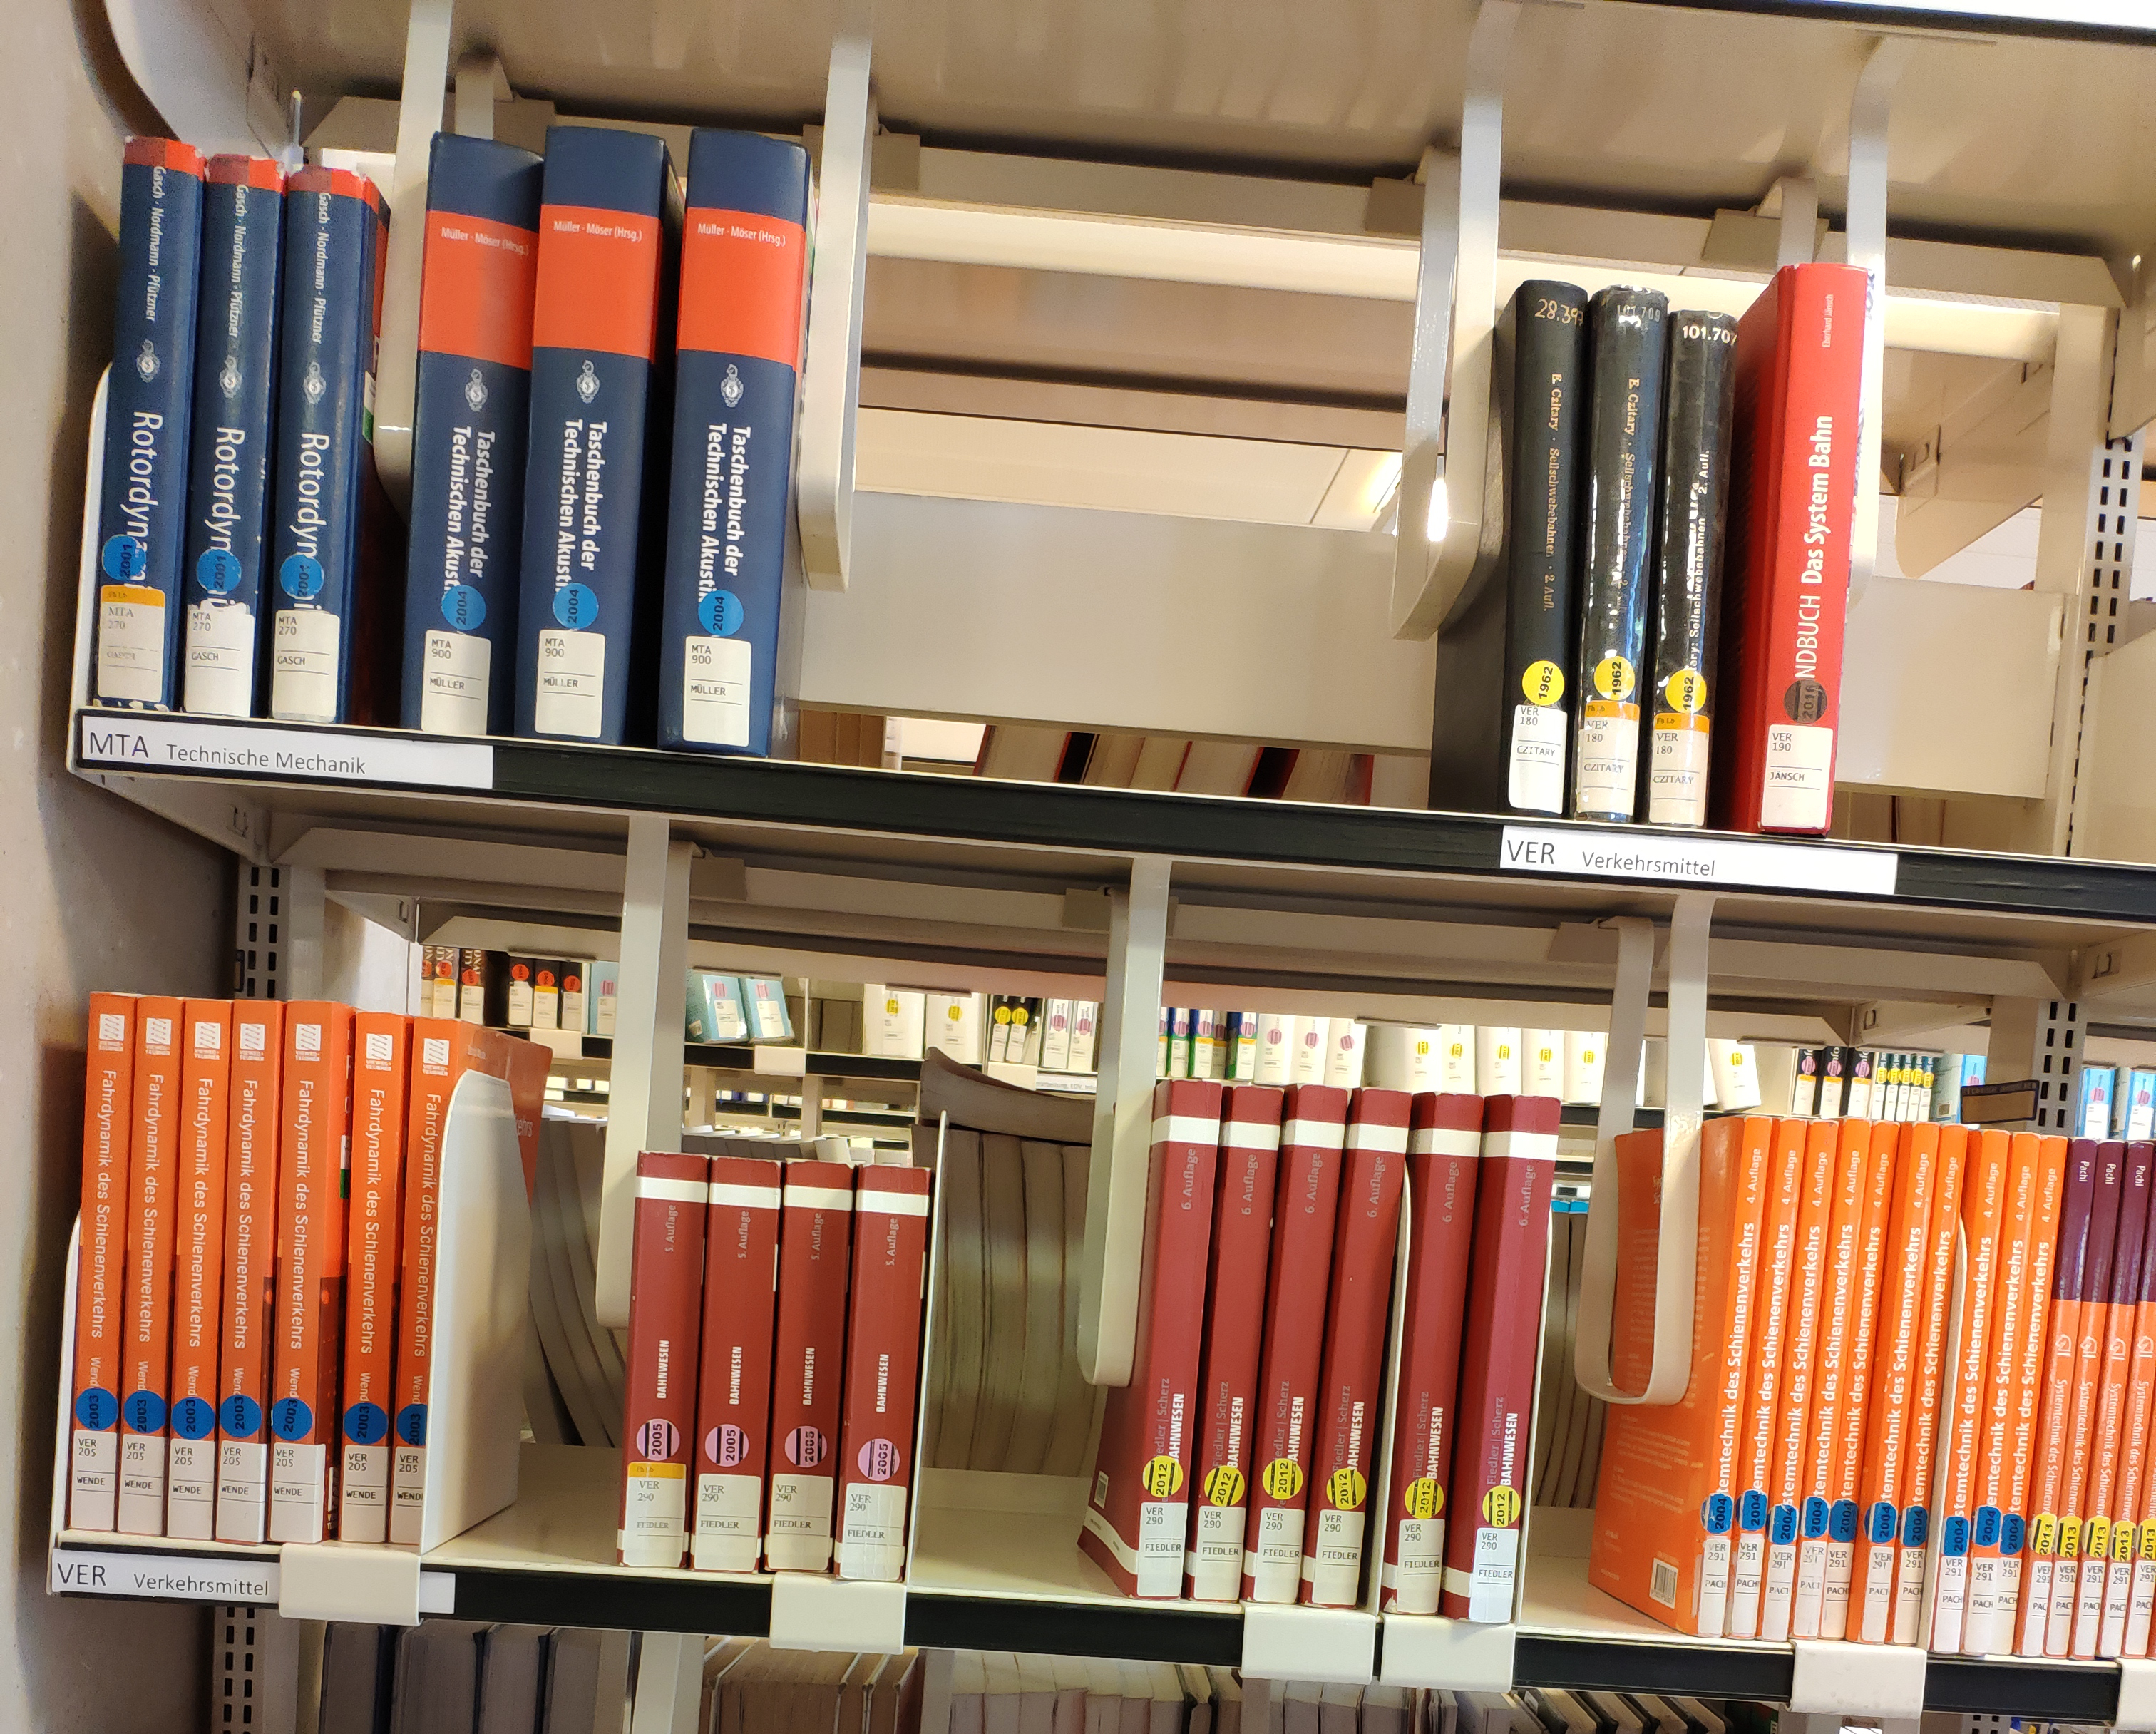
\includegraphics[width=0.4\textwidth]{input.jpg}
 \caption{Input-Bild}
 \label{fig:img}
\end{figure}


\noindent textuell:\\
Strukturierte Klartext-Datei mit Inhalt:
\begin{itemize}
  \item Standort der Bücher (in Büchern zum Ursprung - links-oben)
  \item Vier Pixel-Vektoren, die ein Label in einem Viereck umschließen
\end{itemize}

\subsection{Voraussetzungen und Bedingungen}
\begin{itemize}
  \item Die Bücher müssen gerade (+/- 5°) stehen.
  \item Das Bild darf nicht mehr als 30° von der Waagrechte abweichen.
  \item Das Bild muss eine für die Texterkennung der Labels ausreichende Auflösung aufweisen (Abhängig von der Entfernung).
  \item Das Bild muss farbig sein.
  \item Das Bild muss ausreichend hell sein. 
  \item Ein Weißabgleich muss durchgeführt worden sein.
\end{itemize}

Neue Anforderungen:
\begin{itemize}
  \item Der Hintergrund der Labels muss weiß sein (Intensität muss über dem globalen Otsu-Threshold liegen)
\end{itemize}

\subsection{Methodik}
Methodik- Pipeline
\begin{enumerate}
	\item Hough-Transformation\\
		\textit{Finden der Regalfächer zum Korrigieren der Perspektive}
	\item Persprektivenkorrektur\\tuwe
		\textit{Mittels Transformationsmatrix aus HT berechnet}
	\item Eckenerkennung\\
		\textit{Finden der Ecken von Labels}
	\item Integral imaging\\
		\textit{Finden von Labels innerhalb eines Akzeptanzbereichs, es werden nur Bereiche zwischen verschiedenen, zuvor erkannten, Ecken überprüft}
	\item Eigene Heuristik\\
		\textit{Einordnen von Labels in Buch-Koordinaten}
	\item Optical Character Recognition\\
		\textit{Erkennen von Text auf den Labels in den zuvor erkannten Bereichen}
\end{enumerate}

\subsection{Evaluierungsfragen}
\textbf{Interaktion zwischen den Komponenten:}
\begin{itemize}
	\item \textit{Werden die Regalfächer korrekt erkannt?}\\
		  Voraussetzungen:\tab Seite der Regalfächer, die zur Kamera zeigt, ist schwarz.\\
		  Ergebnis:\tab[2.2cm] An jedem Fach liegt eine Gerade an.
	\item \textit{Wird die Perspektive korrekt angepasst?}\\
		  Voraussetzungen:\tab Korrekte Geraden der Regalfächer.\\
		  Ergebnis:\tab[2.2cm] Bücher und Labels sind im Bild weitestgehend rechteckig.
	\item \textit{Werden alle Labels erkannt?}\\
		  Voraussetzungen:\tab Perspektivenkorrigiertes Bild\\
		  Ergebnis:\tab[2.2cm] Bounding-Boxes der gefundenen Labels
	\item \textit{Sind die Bounding Boxes der gefundenen Labels korrekt? Ist der gesamte Text darin enthalten?}\\
		  Voraussetzungen:\tab Korrekt erkanntes Label oder ein false-positive.\\
		  Ergebnis:\tab[2.2cm] Vier Vektoren, die den gesamten Text umschließen (und nicht mehr). Bei false-positives ist das Ergebnis nicht relevant, jedoch sollte es nicht zu groß sein (z.B. das gesamte Bild überdecken).
	\item \textit{Werden die Labels korrekt in Bücher-Koordinaten umgewandelt?}\\
		  Voraussetzungen:\tab Bounding Boxes der Labels sind korrekt.\\
		  Ergebnis:\tab[2.2cm] Bücher-Koordinatensystem als 2D-Array mit Ursprung links-oben.
	\item \textit{Werden die Labels der TU-Bibliothek korrekt gelesen und in Text umgewandelt?}\\
		  Voraussetzungen:\tab Label Bounding-Boxes wurden korrekt berechnet (enthalten keinen unnötigen Text).\\
		  Ergebnis:\tab[2.2cm] String-Repräsentation des Labels. Erwartete Korrektheit: $>$ 90\% für typische Datensätze.
	\item \textit{Wird die Wahrscheinlichkeit der Label-Korrektheit angemessen berechnet?}\\
		  Voraussetzungen:\tab Korrekt in Text umgewandeltes Label.\\
		  Ergebnis:\tab[2.2cm] Floating-point Wert im Intervall [0, 1]. Alle Labels mit Wahrscheinlichkeit 0 wurden entfernt.
\end{itemize}

\subsection{Zeitplan}
\begin{table}[H]
	\centering
		\begin{tabular}{|c|c|c|}
		\hline
		Meilenstein & abgeschlossen am & Arbeitsaufwand in h\\
		\hline
		Prototyp & 10.11. & 30\\
		\hline
		Hough-Transformation & \st{17.11.} 20.12. & \st{50} 2\\
		\hline
		Perspektivenkorrektur & \st{17.11.} 23.12. & \st{6} 20\\
		\hline
		Labelerkennung & \st{25.11.} 14.11. & 25\\
		\hline
		Labelerkennung - Verbesserungen & \st{25.11.} 5.1. & 30\\
		\hline
		Labels in Buch-Koordinaten & \st{1.12.} 4.1. & \st{4} 0.2\\
		\hline
		Optical Character Recognition & \st{10.12.} 3.1. & \st{110} 40\\
		\hline
		Labels filtern & \st{15.12.} nicht abgeschl. & \st{6} nicht abgeschl.\\
		\hline
		Daten in Output-Format umwandeln & 5.1. & \st{4} 0\\
		\hline
		Tests & \st{18.12.} 5.1. & 5\\
		\hline
		Evaluierung & {20.12.} 5.1. & \st{5} 4 \\
		\hline
		\end{tabular}
\end{table}
%%------------------------------------------------------

%%------------------------------------------------------
\section{Arbeitsteilung}
\begin{center}
  \begin{tabular}{ |l | c | }
    \hline
  Name & Tätigkeiten\\
    \hline
    	Anna Nieto-Berezhinskaya & Harris Eckendetektor (zu feinfühlig und kann deshalb nicht eingesetzt werden)\\
		\hline
		Anand Eichner & houghTransform (+ lokale Funktionen), PerspectiveCorrection (+ lokale Funktionen),\\
		\hline
		Laurenz Edmund Fiala & label\_detection (+ lokale Funktionen),\\
		\hline
		Aleksandar Vucenovic & ocr (+ locals), NCC, SSD\_naive (+ lokale Funktionen),\\
		 & preprocessing (+ lokale Funktionen)\\
		\hline
  \end{tabular}
\end{center}

%%------------------------------------------------------

%%------------------------------------------------------
\section{Methodik}
\subsection{Perspektivenkorrektur:}
Im Vorverarbeitungsschritt wird das Eingabebild in ein Graustufenbild umgewandelt und mit einem vertikalen und einem horizontalen Sobelfilter convoluted um Kantenbilder zu erhalten, dann wird der Betrag dieser Werte genommen um Kanten in beide Richtungen zu finden. Um dem Rauschen im Bild entgegenzuwirken werden alle verbundobjekte unter einer bestimmten Größe ausgefiltert um nur lange Kanten zu behalten. Bei den Vertikalen werden zusätzlich nur die 20 größten Verbundobjekte ausgewählt um dem Rauschen durch die vielen Vertikalen entgegenzuwirken.
Die beiden Kantenbilder werden mit hilfe einer Hough-Transformation in den Parameterraum transformiert. Von dort werden folglich einige Maxmima ausgelesen um einige Geraden im Bild zu ermitteln.
Aus den Linienscharen werden jeweils zwei Vertikale und zwei Horizontale Ausgewählt um ein Rechteck im Raum darzustellen. Die vier Eckpunkte dieses Rechtecks werden vor der geometrischen Verzerrung perspektivisch Korrekt hochskaliert um die unnötige erstellung redundanter Daten zu verhindern. Mit den skalierten Eckpunkten und den eigentlichen Eckpunkten des Bildes wird nun eine perpsektivische Transformationsmatrix gebildet und auf das Bild angewendet.\\

\subsection{Optical Character Recognition:}
\textbf{Image Thresholding (Adaptive):}\\
Das Binarizing des Labels fungiert als Noise Reduktion, zusätzlich ermöglicht es Template Matching mit weiß/schwarzen Bitmaps, da es ein schwarz/weiß Bild zurückliefert.\\

\textbf{Dilation:}\\
Dilation ermöglicht eine korrekte Regionproperties Funktion, da es die Löcher in den Components füllt, und diese damit sauber verbindet.\\

\textbf{Regionprops:}\\
Regionprops gibt uns die Centrtoids und Bounding boxes von collected components, die in unserem Fall potentielle character sind. Die Methode wird benutzt um die Charakter zu segmentieren, in dem man das Originalbild mit den Koordinaten der Bounding Boxes cropped. Zustätzlich verschafft es uns eine Sortiermethode, mithilfe der Centroids können wir die Wörter nämlich richtig von links oben nach rechts unten sortieren,
da Centroids die XY-Koordinaten der Mitte eines Buchstabens im Bild liefert.\\

\textbf{Prewitt Edge-Detection:}\\
Prewitt Edge-Detection wird als preprocessing step für die Dilation und Hough Transformation genutzt, da diese ein Kantenbild als Eingabe brauchen und Prewitt dieses liefert.\\

\textbf{Normalized Cross Correlation (Template Matching):}\\
Der nxcorr/NCC Algorithmus ist ein sehr weit verbreiteter Algorithmus für das Template Matching. In Matlab selbst ist er als normxcorr2-Funktion durchführbar. 
Er wird verwenden, um die korrelation zwischen template und original image zu finden, und normalisiert um richtige Ergebnisse unabhängig von Brightness 
Unterschieden zu liefern. Das Ergebniss ist eine Korrelationsmatrix, die Werte zwischen -1 und 1 enthält, wobei 0 die wenigste Korrelation repräsentiert, 
und 1 die meiste (-1, falls das Original oder Template negiert sind). Wir suchen das globale Maxima in der Matrix, da es den besten Korrelationswert liefert, 
und vergleichen diesen mit allen Werten der Templates. Das Template mit dem höchsten Korrelationswert wird schließlich als matched character weitergegeben.\\

Paper: http://scribblethink.org/Work/nvisionInterface/nip.pdf\\

\textbf{Sum of Squared Differences (Template Matching):}\\
Der SSD Algorithmus wird auch wie der nxcorr2-Algorithmus zum Template Matching verwendet. Der SSD Algorithmus beruht darauf, dass wenn man ein Template 
über das Originalbild legt, und die Summe der quadrierten Differenzen der Pixelwerte bildet, ein möglichst kleiner Wert bei einem match rauskommen sollte (da 
sich die Werte sehr ähnlich sein müssen). Wir haben eine naivere Variante implementiert, da unser Template
und Bild immer gleichgroß sind, und immer beide Bilder die Character zur gänze umschließen, daher müssen wir keine Regionen nach absuchen und offsets ausprobieren.\\
%%------------------------------------------------------
\\

\subsection{Label Detection}

Um die Labels zu erkennen, haben wir uns aufgrund der verschiedenen Label-Dimensionen am Anfang des Projekts dazu entschieden, mittels Integral Imaging (Summed Area Table) zu bestimmen, ob ein Bereich als Label gelten kann oder nicht.\\
Der Prototyp war auch recht erfolgversprechend. Jedoch sind wir im Verlauf des Projekts auf einige Limitationen bei dieser Herangehensweise gestoßen.\\
Es hat sich herausgestellt, dass es oft nicht ganz trivial ist, bei verschiedenen Auflösungen die korrekten Ecken mit dem Harris-Eckendetector zu finden. Hier spielt das Preprocessing, welches ein einfacher Gaußfilter ist, eine große Rolle. Auch die Größe des Gauß-Konvolutionskernels für den Harris-Detektor ist wichtig. Aufgrund von Zeitmangel gegen Ende des Projekts, konnten diese Werte leider nicht mehr so genau bestimmt werden und deshalb ist das Ergebnis leider nicht so genau, wie eigentlich möglich bzw. gewünscht.\\
\\

\textit{Harris-Eckendetektor} \cite{harris}\\
Der Harris-Eckendetektor wird genutzt, um die Ecken der einzelnen Labels zu erkennen.
Ursprünglich war geplant, diese Methode selbst zu implementieren, jedoch war die selbst implementierte Variante zu sensibel und das konnte aufgrund von fehlenden Projektmitgliedern nicht mehr ausgebessert werden.\\
\\

\textit{Summed Area Table / Integral Imaging} \cite{integralimg}\\
Das Integral Imaging wird benutzt, um die Intensität der einzelnen Label-Kandidaten effizient berechnen zu können. Im Programmverlauf wird das genutzt, um das Verhältnis von dunken zu hellen Bildabschnitten zu berechenen und damit bestimmen zu können, ob ein Bereich als Label gelten kann oder nicht.\\
\\

\textit{Otsu-Threshold} \cite{otsu}\\
Es wird ein globaler Threshold benötigt um Labels vom Hintergrund abzugrenzen. Das Integral Image beruht auf dem Ergebnis der Bildmaske dieses Thresholds. Ein Otsu-Threshold eignet sich sehr gut um dynamisch in jedem Bild einen akzeptablen Threshold zu ermitteln.\\
Der Threshold wird auch lokal pro Label-Kandidat angewandt, um den oft sehr hellgrauen Text vom Hintergrund (dem Label) abzugrenzen. Damit ist das Ergebnis des Programms wesentlich zuverlässiger.


%%------------------------------------------------------

%%------------------------------------------------------
\section{Implementierung}
\subsection{Main}
Um das Framwork auszuführen muss main.m mit dem Pfad zum Bild als einziges Argument ausgeführt werden. Die main Funktion gibt dann den json String zurück.
\subsection{Perspektivenkorrektur}
Für die Perspektivenkorrekur ist die PerspectiveCorrection.m Datei zuständig. Diese nutzt einige Builtins für das Preprocessing und eine selbstgeschriebene Implementierung der Hough-Transformation (houghTransform.m). Zum Skalieren der Eckpunkte wurden einige Funktionen implementiert um geometrische Operationen mit Linien in Parameterform durchzuführen. Bei der Hough-Transform wird nur ein Wertebereich von -30 bis +30 Grad genutzt um den Parameterraum möglichst klein zu halten. Weiters wird nur nach 5 Maxima gesucht, dies bietet ein gutes Mittelding zwischen schlechten Ergebnissen und zu wenigen Ergebnissen. Es werden bei den Vertikalen Kanten die jeweils 20 Größten behalten dies bietet auch hier wieder ein gutes Mittelding zu viel Rauschen und einer zu geringen Chance eine gute Kante zu erhalten.
\subsection{Label Detection}
Zuerst werden mit einem Harris-Eckendetektor (MATLAB-builtin) die Ecken im Bild gefunden \cite{harris}. Danach wird ein globaler Otsu-Threshold berechnet \cite{otsu}, der genutzt wird, um eine binäre Bildmaske zu erstellen, wobei alle Pixel mit größerer Intensität als der Threshold, auf 1 gesetzt werden, und alle anderen auf 0.\\
Mit dieser Maske wird wiederum ein Summed Area Table erstellt \cite{integralimg}.\\
Für alle gefundenen Ecken wird nun versucht Nachbarn zu finden, die ein plausibles Label ergeben könnten. Dabei wird aus dem Vorschitt der Persprektivenkorrektur die Höhe der Bücherregale berechnet und daraus die ungefähren Label-Dimensionen abgeleitet. Diese onstanten Umrechnungsfaktoren wurden durch analysieren von Bildern abgelesen und fix in das Programm eingetragen. So ist zum Beispiel der Faktor von Regalhöhe zu Labelhöhe 0.135.\\
Für alle gefundenen Ecken-Nachbar-Kombinationen wird nun überprüft, ob der Schwarzanteil dem eines typischen Labels entsprcht. Dafür wird ein lokaler Otsu-Threshold berechnet, der den Label-Text vom Hintergrund trennt. Mit diesem . Im Falle eines schrägen Labels, werden mittels der MATLAB-Funktion "imclearborder" eventuell vorhandene Ränder ignoriert. Dann wird mit dieser Maske die anzahl an schwarzen Pixeln summiert und in Verhältnis zu dem Ergebnis des Integral Imaging (weiße Bildteile) verglichen. Wenn dieser Wert im Akzeptanzbereich liegt, nehmen wir an, im Bereich zwischen der Ecke-Nachbar-Kombination befindet sich ein Label.\\
\\
\\
%%------------------------------------------------------

%%------------------------------------------------------
\section{Evaluierung}
(2-X Seiten)\\
Hier stellt ihr Euren Datensatz vor und beantwortet Evaluierungsfragen:\\
\subsection{Datensatz}
Insgesamt 14 Bilder der Bücherregale aus der Unibibliothek alle mit einem Xiaomi Mi MIX 2S aufgenommen.\\
Auflösung : 4032 x 3024\\
Diskussion der Evaluierungsfragen: Beantwortung der Fragen, Diskussion anhand von Beispielen, Diskussion von Grenzfällen: für welche Bilder funktioniert die Implementierung, für welche nicht? Worin unterscheiden sich diese Bilder? Warum funktionieren sie nicht? etc.\\
Evaluiert wird der ganze Datensatz, nicht nur einzelne Bilder. Einzelne Bilder können zum Aufzeigen von Fehlern/Problemen/besonders guten Ergebnissen... genutzt werden.\\
Zur Evaluierung gehört auch das Testen der einzelnen Methodiken (separat), mit Erwähnung eventueller Einschränkungen.
%%------------------------------------------------------

%%------------------------------------------------------
\section{Schlusswort}
(max. 1 Seite)\\
Hier fasst ihr Ergebnisse Eures Projekt zusammen:\\
Welche Schlussfolgerung lässt sich ziehen? Gibt es offene Probleme? Wie lässt sich Eure Lösung noch verbessern? etc.
%%------------------------------------------------------

%%------------------------------------------------------
\bibliographystyle{plain}
\bibliography{edbv_lit}
%%Bei verwendung von Latex schreibt ihr eure Referenzen in ein eigenes bib-File (siehe hier edbv_lit.bib). Jene Referenzen, die ihr im Bericht mittels \cite zitiert, werden automatisch in die Referenzliste übernommen. Weitere Information zum Einbinden von BibTex gibt es hier: http://www.bibtex.org/Using/de/
%%------------------------------------------------------
\textbf{Webseiten werden als Fußzeilen (an jener Stelle wo sie verwendet werden) eingebunden, nicht als Literature!}

\end{document}
\grid
\grid
